
%{{第二十七回}}{第二十七回}}

\chapter{滴翠亭杨妃戏彩蝶\\埋香冢飞燕泣残红}\label{part0031_split_000.htmlux5cux23calibre_pb_0}

{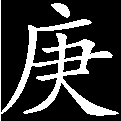
\includegraphics[width=3mm]{../Images/00004}《葬花吟》是大观园诸艳之归源小引,故用在饯花日诸艳毕集之期。饯花日不论其典与不典,只取其韵耳。}

话说林黛玉正自悲泣,忽听院门响处,只见宝钗出来了,宝玉、袭人一群人送了出来。待要上去问着宝玉,又恐当着众人问,羞了他倒不便,因而闪过一旁,让宝钗去了,宝玉等进去关了门,方转过来,犹望着门洒了几点泪。{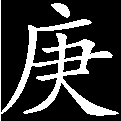
\includegraphics[width=3mm]{../Images/00004}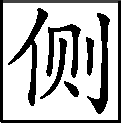
\includegraphics[width=3mm]{../Images/00011}\footnotesize \kaishu 四字闪煞颦儿也。}自觉无味,便转身回来,无精打彩的卸了残妆。

紫鹃、雪雁素日知道他的情性:无事闷坐,不是愁眉,{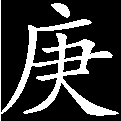
\includegraphics[width=3mm]{../Images/00004}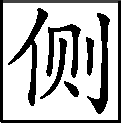
\includegraphics[width=3mm]{../Images/00011}\footnotesize \kaishu 画美人之秘诀。}便是长叹,且好端端的不知为了什么,便常常的就自泪自干。{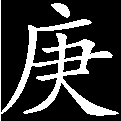
\includegraphics[width=3mm]{../Images/00004}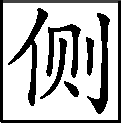
\includegraphics[width=3mm]{../Images/00011}\footnotesize \kaishu 补写,却是避繁文法。}先时还解劝,怕他思父母,想家乡,受了委曲,用话来宽慰解劝。谁知后来一年一月竟常常的如此,{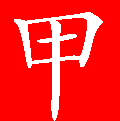
\includegraphics[width=3mm]{../Images/00002}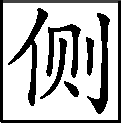
\includegraphics[width=3mm]{../Images/00011}\footnotesize \kaishu 补潇湘馆常文也。}把这个样儿看惯了,也都不理论了。所以没人去理,由他去闷坐,{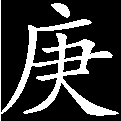
\includegraphics[width=3mm]{../Images/00004}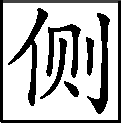
\includegraphics[width=3mm]{../Images/00011}\footnotesize \kaishu 所谓``久病床前少孝子''是也。}只管睡觉去了。那林黛玉倚着床栏杆,两手抱着膝,{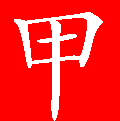
\includegraphics[width=3mm]{../Images/00002}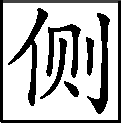
\includegraphics[width=3mm]{../Images/00011}\footnotesize \kaishu 画美人秘诀。}眼睛含着泪,{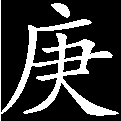
\includegraphics[width=3mm]{../Images/00004}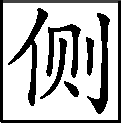
\includegraphics[width=3mm]{../Images/00011}\footnotesize \kaishu 前批的画美人秘诀,今竟画出《金闺夜坐图》来了。}好似木雕泥塑{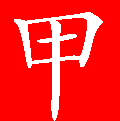
\includegraphics[width=3mm]{../Images/00002}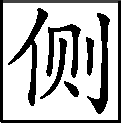
\includegraphics[width=3mm]{../Images/00011}\footnotesize \kaishu 木是旃檀,泥是金沙方可。}的一般,直坐到三更多天方才睡了。一宿无话。

至次日,乃是四月二十六日,原来这日未时交芒种节。尚古风俗:凡交芒种节的这日,都要设摆各色礼物,祭饯花神,言芒种一过,便是夏日了,众花皆卸,花神退位,{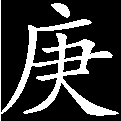
\includegraphics[width=3mm]{../Images/00004}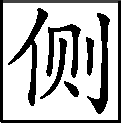
\includegraphics[width=3mm]{../Images/00011}\footnotesize \kaishu 无论事之有无,看去有理。}须要饯行。然闺中更兴这件风俗,所以大观园中之人都早起来了。那些女孩子,或用花瓣柳枝编成轿马的,或用绫锦纱罗叠成干旄旌幢的,都用彩线系了。每一颗树每一枝花上,都系上了这些物事。满园中绣带飘飖,花枝招展,{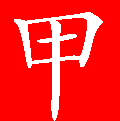
\includegraphics[width=3mm]{../Images/00002}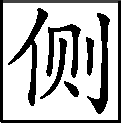
\includegraphics[width=3mm]{../Images/00011}\footnotesize \kaishu 数句大观园景,倍胜省亲一回,在一园人俱得闲闲寻乐上看,彼时只有元春一人闲耳。 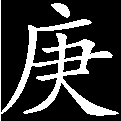
\includegraphics[width=3mm]{../Images/00004}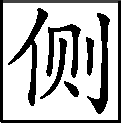
\includegraphics[width=3mm]{../Images/00011}\footnotesize \kaishu 数句抵省亲一回文字,反觉闲闲有趣有味的领略。}更又兼这些人打扮得桃羞杏让,燕妒莺惭,{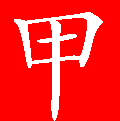
\includegraphics[width=3mm]{../Images/00002}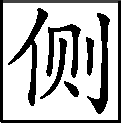
\includegraphics[width=3mm]{../Images/00011}\footnotesize \kaishu 桃杏、燕莺是这样用法。}一时也道不尽。

且说宝钗、迎春、探春、惜春、李纨、凤姐{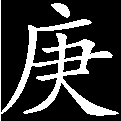
\includegraphics[width=3mm]{../Images/00004}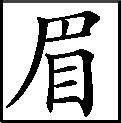
\includegraphics[width=3mm]{../Images/00010}\footnotesize \kaishu 写凤姐随大众一笔,不见红玉一段则认为泛文矣。何一丝不漏若此。畸笏。}等并巧姐、大姐\href{../Text/part0031_split_000.html\#lnkback_1_a}{\textsuperscript{①}}、香菱与众丫鬟们都在园内顽耍,独不见林黛玉。迎春因说道:``林妹妹怎么不见?好个懒丫头!这会子还睡觉不成?''宝钗道:``你们等着,我去闹了他来。''说着便丢下众人,一直的往潇湘馆来。正走着,只见文官等十二个女孩子也来了,{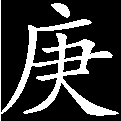
\includegraphics[width=3mm]{../Images/00004}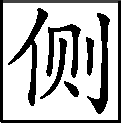
\includegraphics[width=3mm]{../Images/00011}\footnotesize \kaishu 一人不漏。}见宝钗问了好,说了一回闲话。宝钗回身指道:``他们都在那里呢,你们找去罢。我叫林姑娘去就来。''说着便往潇湘馆来。{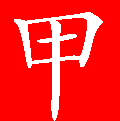
\includegraphics[width=3mm]{../Images/00002}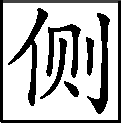
\includegraphics[width=3mm]{../Images/00011}\footnotesize \kaishu 安插一处,好写一处,正一张口难说两家话也。}忽然抬头见宝玉进去了,宝钗便站住,低头想了一想:宝玉和林黛玉是从小一处长大,他二人间多有不避嫌疑之处,嘲笑喜怒无常;{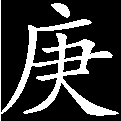
\includegraphics[width=3mm]{../Images/00004}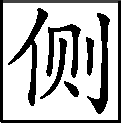
\includegraphics[width=3mm]{../Images/00011}\footnotesize \kaishu 道尽二玉连日事。}况且黛玉素习猜忌,好弄小性儿。此刻自己也进去,一则宝玉不便,二则黛玉嫌疑,{{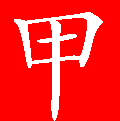
\includegraphics[width=3mm]{../Images/00002}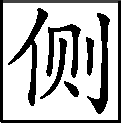
\includegraphics[width=3mm]{../Images/00011}\footnotesize \kaishu 道尽黛玉每每小性,全不在宝钗{(身)}{[}心{]}上。}}倒是回来的妙。

想毕,抽身要寻别的姊妹去,忽见前面一双玉色蝴蝶,大如团扇,一上一下的迎风翩跹,十分有趣。宝钗意欲扑了来顽耍,遂向袖中取出扇子来,向草地下来扑。{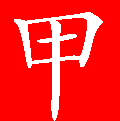
\includegraphics[width=3mm]{../Images/00002}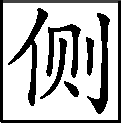
\includegraphics[width=3mm]{../Images/00011}\footnotesize \kaishu 可是一味知书识礼女夫子行止?写宝钗无不相宜。}只见那一双蝴蝶忽起忽落,来来往往,穿花度柳,将欲过河。倒引的宝钗蹑手蹑脚的,一直跟到池中的滴翠亭,香汗淋漓,娇喘细细,{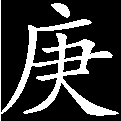
\includegraphics[width=3mm]{../Images/00004}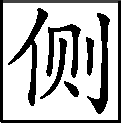
\includegraphics[width=3mm]{../Images/00011}\footnotesize \kaishu 若玉兄在,必有许多张罗。}也无心扑了。{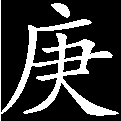
\includegraphics[width=3mm]{../Images/00004}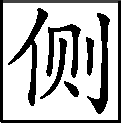
\includegraphics[width=3mm]{../Images/00011}\footnotesize \kaishu 原是无可无不可。}刚欲回来,只听亭子里面嘁嘁喳喳有人说话。{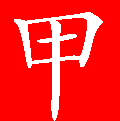
\includegraphics[width=3mm]{../Images/00002}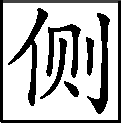
\includegraphics[width=3mm]{../Images/00011}\footnotesize \kaishu 无闲纸闲笔之文如此。}原来这亭子四面俱是游廊曲桥,盖在池中,周围都是雕镂槅子糊着纸。

宝钗在亭外听见说话,便站住往里细听,{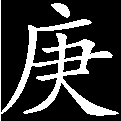
\includegraphics[width=3mm]{../Images/00004}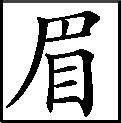
\includegraphics[width=3mm]{../Images/00010}\footnotesize \kaishu 这桩风流案,又一体写法,甚当。己卯冬夜。}只听说道:``你瞧瞧这手帕子,果然是你丢的那块,你就拿着;要不是,就还芸二爷去。''又有一人道:``可不是那块!拿来给我罢。''又听说道:``你拿什么谢我呢?难道白寻了来不成。''又答道:``我既许了谢你,自然不哄你。''又听说道:``我寻了来给你,自然谢我;但只是拣的人,你就不拿什么谢他?''又回道:``你别胡说。他是个爷们家,拣了我们的东西,自然该还的。叫我拿什么给他呢?''又听说道:``你不谢他,我怎么回他呢?况且他再三再四的和我说了,若没谢的,不许给你呢。''半晌,又听答道:``也罢,拿我这个给他,就算谢他的罢。------你要告诉别人呢?须说个誓来。''又听说道:``我要告诉一个人,就长一个疔,日后不得好死!''又听说道:``嗳呀!咱们只顾说话,看有人来悄悄的在外头听见。{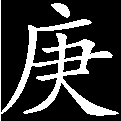
\includegraphics[width=3mm]{../Images/00004}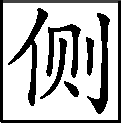
\includegraphics[width=3mm]{../Images/00011}\footnotesize \kaishu 岂敢。 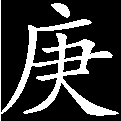
\includegraphics[width=3mm]{../Images/00004}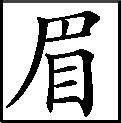
\includegraphics[width=3mm]{../Images/00010}\footnotesize \kaishu 这是自难自法,好极好极!◇惯用险笔如此。壬午夏,雨窗。}不如把这槅子都推开了,{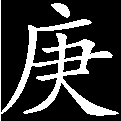
\includegraphics[width=3mm]{../Images/00004}\includegraphics[width=3mm]{../Images/00011}\footnotesize \kaishu 贼起飞志,不假。}便是有人见咱们在这里,他们只当我们说顽话呢。若走到跟前,咱们也看的见,就别说了。''

宝钗在外面听见这话,心中吃惊,{\includegraphics[width=3mm]{../Images/00002}\includegraphics[width=3mm]{../Images/00011}\footnotesize \kaishu 四字写宝钗守身如此。}想道:``怪道从古至今那些奸淫狗盗的人,心机都不错。{\includegraphics[width=3mm]{../Images/00004}\includegraphics[width=3mm]{../Images/00011}\footnotesize \kaishu 道尽矣。}这一开了,见我在这里,他们岂不臊了。况才说话的语音儿,大似宝玉房里的红儿。他素习眼空心大,最是个头等刁钻古怪的东西。今儿我听了他的短儿,一时人急造反,狗急跳墙,不但生事,而且我还没趣。如今便赶着躲了,料也躲不及,少不得要使个`金蝉脱壳'的法子。''犹未想完,只听``咯吱''一声,宝钗便故意放重了脚步,{\includegraphics[width=3mm]{../Images/00004}\includegraphics[width=3mm]{../Images/00011}\footnotesize \kaishu 闺中弱女机变,如此之便,如此之急。}笑着叫道:``颦儿,我看你往那里藏!''一面说,一面故意往前赶。那亭子里的红玉、坠儿刚一推窗,只见宝钗如此说着往前赶,{\includegraphics[width=3mm]{../Images/00004}\includegraphics[width=3mm]{../Images/00010}\footnotesize \kaishu 此句实借红玉反写宝钗也,勿得认错作者章法。}两个人都唬怔了。宝钗反向他二人笑道:``你们把林姑娘藏在那里了?''{\includegraphics[width=3mm]{../Images/00004}\includegraphics[width=3mm]{../Images/00011}\footnotesize \kaishu 像极!好煞,妙煞!焉得不拍案叫绝!}坠儿道:``何曾见林姑娘了。''宝钗道:``我才在河边看着他在这里蹲着弄水儿的。我要悄悄的唬他一跳,还没走到跟前,他倒看见我了,朝东一绕就不见了。必是藏在这里头了。''{\includegraphics[width=3mm]{../Images/00004}\includegraphics[width=3mm]{../Images/00011}\footnotesize \kaishu 像极!是极!}一面说,一面故意进去寻了一寻,抽身就走,{\includegraphics[width=3mm]{../Images/00004}\includegraphics[width=3mm]{../Images/00011}\footnotesize \kaishu 像极!是极!}口里说道:``一定又是在那山子洞里去。遇见蛇,咬一口也罢了。''一面说一面走,心里又好笑:{\includegraphics[width=3mm]{../Images/00002}\includegraphics[width=3mm]{../Images/00011}\footnotesize \kaishu 真弄婴儿,轻便如此,即余至此亦要发笑。}这件事算遮过去了,不知他二人是怎么样。

谁知红玉听见了宝钗的话,便信以为真,{\includegraphics[width=3mm]{../Images/00002}\includegraphics[width=3mm]{../Images/00011}\footnotesize \kaishu 宝钗身份。 \includegraphics[width=3mm]{../Images/00004}\includegraphics[width=3mm]{../Images/00011}\footnotesize \kaishu 实有这一句的。}让宝钗去远,便拉坠儿道:``了不得了!林姑娘蹲在这里,一定听了话去了!''{\includegraphics[width=3mm]{../Images/00004}\includegraphics[width=3mm]{../Images/00011}\footnotesize \kaishu 移东挪西,任意写去,却是真有的。}坠儿听说,也半日不言语。红玉又道:``这可怎么样呢?''{\includegraphics[width=3mm]{../Images/00002}\includegraphics[width=3mm]{../Images/00011}\footnotesize \kaishu 二句系黛玉身份。}坠儿道:``便听见了,管谁筋疼,各人干各人的就完了。''{\includegraphics[width=3mm]{../Images/00004}\includegraphics[width=3mm]{../Images/00011}\footnotesize \kaishu 勉强话。}红玉道:``若是宝姑娘听见,还倒罢了。林姑娘嘴里又爱刻薄人,心里又细,他一听见了,倘或走露了,怎么样呢?''二人正说着,只见文官、香菱、司棋、待书等上亭子来了。二人只得掩住这话,且和他们顽笑。

只见凤姐儿站在山坡上招手叫红玉,红玉连忙弃了众人,跑至凤姐前,笑问:``奶奶使唤作什么?''凤姐打量了一打量,见他生的干净俏丽,说话知趣,因说道:``我的丫头今儿没跟进来。我这会子想起一件事来,要使唤个人出去,可不知你能干不能干,说的齐全不齐全?''红玉道:``奶奶有什么话,只管吩咐我说去。若说不齐全,误了奶奶的事,凭奶奶责罚罢了。''{\includegraphics[width=3mm]{../Images/00002}\includegraphics[width=3mm]{../Images/00011}\footnotesize \kaishu 操必胜之券。红儿机括志量,自知能应阿凤使令意。}凤姐笑道:``你是谁房里的?{\includegraphics[width=3mm]{../Images/00004}\includegraphics[width=3mm]{../Images/00011}\footnotesize \kaishu 反如此问。}我使你出去,他回来找你,我好替你答应。''{\includegraphics[width=3mm]{../Images/00004}\includegraphics[width=3mm]{../Images/00011}\footnotesize \kaishu 问那小姐为此。}红玉道:``我是宝二爷房里的。''凤姐听了笑道:``嗳哟!你原来是宝玉房里的,怪道呢。{\includegraphics[width=3mm]{../Images/00002}\includegraphics[width=3mm]{../Images/00011}\footnotesize \kaishu ``哎哟''``怪道''四字,一是玉兄手下无能为者。前文打量生的``干净俏丽''四字,合而观之,小红则活现于纸上矣。 \includegraphics[width=3mm]{../Images/00004}\includegraphics[width=3mm]{../Images/00011}\footnotesize \kaishu 夸赞语也。}也罢了,你到我家,告诉你平姐姐:外头屋里桌子上汝窑盘子架儿底下放着一卷银子,那是一百二十两,给绣匠的工价,等张材家的来要,当面称给他瞧了,再给他拿去。{\includegraphics[width=3mm]{../Images/00004}\includegraphics[width=3mm]{../Images/00011}\footnotesize \kaishu 一件。}再里头屋里床上有个小荷包,拿了来给我。''{\includegraphics[width=3mm]{../Images/00004}\includegraphics[width=3mm]{../Images/00011}\footnotesize \kaishu 二件。}

红玉听了,撤身去了。回来只见凤姐不在这山坡上了。因见司棋从山洞里出来,站着系裙子,{\includegraphics[width=3mm]{../Images/00004}\includegraphics[width=3mm]{../Images/00011}\footnotesize \kaishu 小点缀。一笑。}便上来问道:``姐姐,不知道二奶奶往那去了?''司棋道:``没理论。''{\includegraphics[width=3mm]{../Images/00004}\includegraphics[width=3mm]{../Images/00011}\footnotesize \kaishu 妙极!}红玉听了,又往四下里看,只见那边探春、宝钗在池边看鱼。红玉便走来陪笑问道:``姑娘们可看见二奶奶没有?''探春道:``往大奶奶院里找去。''红玉听了,才往稻香村来,顶头只见{\includegraphics[width=3mm]{../Images/00004}\includegraphics[width=3mm]{../Images/00011}\footnotesize \kaishu 又一折。}晴雯、绮霰、碧痕、紫绡、麝月、待书、入画、莺儿等一群人来了。晴雯一见了红玉,便说道:``你只是疯罢!花儿也不浇,雀儿也不喂,茶炉子也不爖,就在外头逛。''{\includegraphics[width=3mm]{../Images/00004}\includegraphics[width=3mm]{../Images/00011}\footnotesize \kaishu 必有此数句,方引出称心得意之语来。再不用本院人见小红,此差只几分遂心。}红玉道:``昨儿二爷说了,今儿不用浇花,过一日再浇罢。我喂雀儿的时候,姐姐还睡觉呢。''碧痕道:``茶炉子呢?''{\includegraphics[width=3mm]{../Images/00002}\includegraphics[width=3mm]{../Images/00011}\footnotesize \kaishu 岔一人问,俱是不受用意。}红玉道:``今儿不是我爖的班儿,有茶没茶别问我。''绮霰道:``你听听他的嘴!你们别说了,让他逛去罢。''红玉道:``你们再问问我逛了没有。二奶奶才使唤我说话取东西去的。''{\includegraphics[width=3mm]{../Images/00002}\includegraphics[width=3mm]{../Images/00011}\footnotesize \kaishu 非小红夸耀,系尔等逼出来的,离怡红意已定矣。}说着将荷包举给他们看,{\includegraphics[width=3mm]{../Images/00004}\includegraphics[width=3mm]{../Images/00011}\footnotesize \kaishu 得意!称心如意,在此一举荷包。}方没言语了,{\includegraphics[width=3mm]{../Images/00002}\includegraphics[width=3mm]{../Images/00011}\footnotesize \kaishu 众女儿何苦自讨之。}大家分路走开。晴雯冷笑道:``怪道呢!原来爬上高枝儿去了,把我们不放在眼里。不知说了一句半句话,名儿姓儿知道了不曾呢,就把他兴的这样!这一遭儿半遭儿的算不得什么,过了后儿还得听呵!有本事的从今儿出了这园子,长长远远的在高枝儿上才算得。''{{\includegraphics[width=3mm]{../Images/00004}\includegraphics[width=3mm]{../Images/00011}\footnotesize \kaishu 虽是醋语,却{(与)}{[}过{]}下无痕。}}一面说着走了。

这里红玉听说,也不便分证,只得忍着气来找凤姐。到了李氏房中,果见凤姐在那里说话儿呢。红玉便上来回道:``平姐姐说,奶奶刚出来了,他就把银子收起来了,{\includegraphics[width=3mm]{../Images/00002}\includegraphics[width=3mm]{../Images/00011}\footnotesize \kaishu 交代不在盘架下了。}才张材家的来取,当面称了给他拿去了。''说着将荷包递了上去,{\includegraphics[width=3mm]{../Images/00004}\includegraphics[width=3mm]{../Images/00011}\footnotesize \kaishu 两件完了。}又道:``平姐姐叫我回奶奶:旺儿进来讨奶奶的示下,好往那家子去的。平姐姐就把这话按着奶奶的主意打发他去了。''凤姐笑道:``他怎么按我的主意打发去了?''{\includegraphics[width=3mm]{../Images/00002}\includegraphics[width=3mm]{../Images/00011}\footnotesize \kaishu 可知前红玉云``就把那按奶奶的主意'',``主意''是欲俭,但恐累赘耳,故阿凤有是问,彼能细答。}红玉道:``平姐姐说:我们奶奶问这里奶奶好。原是我们二爷不在家,虽然迟了两天,只管请奶奶放心。等五奶奶{\includegraphics[width=3mm]{../Images/00002}\includegraphics[width=3mm]{../Images/00011}\footnotesize \kaishu 又一门。}好些,我们奶奶还会了五奶奶来瞧奶奶呢。五奶奶前儿打发人来说,舅奶奶{\includegraphics[width=3mm]{../Images/00002}\includegraphics[width=3mm]{../Images/00011}\footnotesize \kaishu 又一门。}带了信来了,问奶奶好,还要和这里的姑奶奶{\includegraphics[width=3mm]{../Images/00002}\includegraphics[width=3mm]{../Images/00011}\footnotesize \kaishu 又一门。}寻两丸延年神验万全丹。若有了,奶奶打发人来,只管送在我们奶奶这里。明儿有人去,就顺路给那边舅奶奶带去的。''

话未说完,李纨笑道:``嗳哟哟!这话我就不懂了。{\includegraphics[width=3mm]{../Images/00002}\includegraphics[width=3mm]{../Images/00011}\footnotesize \kaishu 红玉今日方遂心如意,却为宝玉后伏线。 \includegraphics[width=3mm]{../Images/00004}\includegraphics[width=3mm]{../Images/00011}\footnotesize \kaishu 又一润色。}什么`奶奶'`爷爷'的一大堆。''凤姐笑道:``怨不得你不懂,这是四五门子的话呢。''说着又向红玉笑道:``好孩子,倒难为你说的齐全。别像他们扭扭捏捏蚊子似的。{\includegraphics[width=3mm]{../Images/00004}\includegraphics[width=3mm]{../Images/00011}\footnotesize \kaishu 写死假斯文。}嫂子不知道,如今除了我随手使的这几个人之外,我就怕和别人说话。他们必定把一句话拉长了作两三截儿,咬文咬字,拿着腔,哼哼唧唧的,急的我冒火。先时我们平儿也是这么着,我就问着他:必定装蚊子哼哼,难道就是美人了?{\includegraphics[width=3mm]{../Images/00004}\includegraphics[width=3mm]{../Images/00011}\footnotesize \kaishu 贬杀,骂杀。}说了几遭才好些了。''李宫裁笑道:``都像你破落户才好。''凤姐又道:``这个丫头就好。{\includegraphics[width=3mm]{../Images/00002}\includegraphics[width=3mm]{../Images/00011}\footnotesize \kaishu 红玉听见了么?}方才说话虽不多,听那口气就简断。''{\includegraphics[width=3mm]{../Images/00002}\includegraphics[width=3mm]{../Images/00011}\footnotesize \kaishu 红玉此刻心内想:可惜晴雯等不在傍。}说着又向红玉笑道:``你明儿伏侍我去罢。我认你作女儿,我再调理调理,你就出息了。''{\includegraphics[width=3mm]{../Images/00004}\includegraphics[width=3mm]{../Images/00011}\footnotesize \kaishu 不假。}

红玉听了,扑哧一笑。凤姐道:``你怎么笑?你说我年轻,比你能大几岁,就作你的妈了?你别作春梦呢!你打听打听,这些人都比你大的大的,赶着我叫妈,我还不理呢!''红玉笑道:``我不是笑这个,我笑奶奶认错了辈数了。我妈是奶奶的女儿,{\includegraphics[width=3mm]{../Images/00004}\includegraphics[width=3mm]{../Images/00011}\footnotesize \kaishu 所以说``比你大的大的''。}这会子又认我作女儿。''凤姐道:``谁是你妈?''{\includegraphics[width=3mm]{../Images/00004}\includegraphics[width=3mm]{../Images/00011}\footnotesize \kaishu 晴雯说过。}李宫裁道:``你原来不认得他?他就是林之孝之女。''{\includegraphics[width=3mm]{../Images/00002}\includegraphics[width=3mm]{../Images/00011}\footnotesize \kaishu 管家之女,而晴卿辈挤之,招祸之媒也。}凤姐听了十分诧异,因笑道:``哦!原来是他的丫头。''{\includegraphics[width=3mm]{../Images/00002}\includegraphics[width=3mm]{../Images/00011}\footnotesize \kaishu 传神。}又笑道:``林之孝两口子都是锥子扎不出一声儿来的。我成日家说,他们倒是配就了的一对,夫妻一双天聋地哑。{\includegraphics[width=3mm]{../Images/00002}\includegraphics[width=3mm]{../Images/00011}\footnotesize \kaishu 用的是阿凤口角。}那里承望养出这么个伶俐丫头来!你十几岁了?''红玉道:``十七岁了。''又问名字,{\includegraphics[width=3mm]{../Images/00002}\includegraphics[width=3mm]{../Images/00011}\footnotesize \kaishu 真真不知名,可叹!}红玉道:``原叫红玉的,因为重了宝二爷,如今叫红儿了。''

凤姐听了将眉一皱,把头一回,说道:``讨人嫌的很!{\includegraphics[width=3mm]{../Images/00004}\includegraphics[width=3mm]{../Images/00011}\footnotesize \kaishu 又一下针。}得了玉的益似的,你也玉,我也玉。''因说道:``既这么着,上月\href{../Text/part0031_split_000.html\#lnkback_2_a}{\textsuperscript{②}}我还和他妈说,`赖大家的如今事多,也不知这府里谁是谁,你替我好好的挑两个丫头我使',他一般的答应。他饶不挑,倒把他这女孩子送了别处去。难道跟我必定不好?''李氏笑道:``你可是又多心了。他进来在先,你说话在后,怎么怨得他妈呢!''凤姐道:``既这么着,明儿我和宝玉说,叫他再要人,{\includegraphics[width=3mm]{../Images/00002}\includegraphics[width=3mm]{../Images/00011}\footnotesize \kaishu 有悌弟之心。}叫这丫头跟我去。可不知本人愿意不愿意?''{\includegraphics[width=3mm]{../Images/00002}\includegraphics[width=3mm]{../Images/00011}\footnotesize \kaishu 总是追写红玉十分心事。}红玉笑道:``愿意不愿意,我们不敢说。{\includegraphics[width=3mm]{../Images/00002}\includegraphics[width=3mm]{../Images/00011}\footnotesize \kaishu 好答!可知两处俱是主儿。 \includegraphics[width=3mm]{../Images/00004}\includegraphics[width=3mm]{../Images/00011}\footnotesize \kaishu 有话。好答。}只是跟着奶奶,我们也学些眉眼高低,{\includegraphics[width=3mm]{../Images/00004}\includegraphics[width=3mm]{../Images/00011}\footnotesize \kaishu 千愿意万愿意之言。}出入上下,大小的事也得见识见识。''{\includegraphics[width=3mm]{../Images/00002}\includegraphics[width=3mm]{../Images/00011}\footnotesize \kaishu 且系本心本意,``狱神庙''回内方见。 \includegraphics[width=3mm]{../Images/00004}\includegraphics[width=3mm]{../Images/00010}\footnotesize \kaishu 奸邪婢岂是怡红应答者,故即逐之。前良儿,后篆儿,便是确证。作者又不得可也。己卯冬夜。 \includegraphics[width=3mm]{../Images/00004}\includegraphics[width=3mm]{../Images/00010}\footnotesize \kaishu 此系未见``抄没''、``狱神庙''诸事,故有是批。丁亥夏。畸笏。}刚说着,只见王夫人的丫头来请,{\includegraphics[width=3mm]{../Images/00004}\includegraphics[width=3mm]{../Images/00011}\footnotesize \kaishu 截得真好。}凤姐便辞了李宫裁去了。红玉回怡红院,{\includegraphics[width=3mm]{../Images/00004}\includegraphics[width=3mm]{../Images/00011}\footnotesize \kaishu 好,接得更好。}不在话下。

如今且说林黛玉因夜间失寐,次日起迟了,闻得众姊妹都在园中作饯花会,恐人笑他痴懒,连忙梳洗了出来。刚到了院中,只见宝玉进门来了,笑道:``好妹妹,昨儿可告我不曾?{\includegraphics[width=3mm]{../Images/00002}\includegraphics[width=3mm]{../Images/00011}\footnotesize \kaishu 明知无是事,不得不作开谈。}叫我悬了一夜心。''{\includegraphics[width=3mm]{../Images/00004}\includegraphics[width=3mm]{../Images/00011}\footnotesize \kaishu 并不为告悬心。}林黛玉便回头叫紫鹃道:{\includegraphics[width=3mm]{../Images/00002}\includegraphics[width=3mm]{../Images/00011}\footnotesize \kaishu 不见宝玉,阿颦断无此一段闲言,总在欲言不言难禁之意,了却``情情''之正文也。 \includegraphics[width=3mm]{../Images/00004}\includegraphics[width=3mm]{../Images/00011}\footnotesize \kaishu 倒像不曾听见的。}``把屋子收拾了,下一扇纱屉子;看那大燕子回来,把帘子放下来,拿狮子倚住;烧了香,就把炉罩上。''一面说一面仍往外走。宝玉见他这样,还认作是昨日中晌的事,{\includegraphics[width=3mm]{../Images/00002}\includegraphics[width=3mm]{../Images/00011}\footnotesize \kaishu 毕真,不错。}那知晚间的这段公案,还打恭作揖的。黛玉正眼也不看,各自出了院门,一直找别的姊妹去了。宝玉心中纳闷,自己猜疑:看起这个光景来,不像是为昨日的事;但只昨日我回来的晚了,又没见他,再没有冲撞了他的去处。{\includegraphics[width=3mm]{../Images/00004}\includegraphics[width=3mm]{../Images/00011}\footnotesize \kaishu 毕真,不错。}一面想,一面走,又由不得从后面追了来。

只见宝钗、探春正在那边看仙鹤,{\includegraphics[width=3mm]{../Images/00004}\includegraphics[width=3mm]{../Images/00011}\footnotesize \kaishu 二玉文字岂是容易写的,故有此截。 \includegraphics[width=3mm]{../Images/00004}\includegraphics[width=3mm]{../Images/00010}\footnotesize \kaishu 《石头记》用截法、岔法、突然法、伏线法、由近渐远法、将繁改简法、重作轻抹法、虚敲实应法种种诸法,总在人意料之外,且不曾见一丝牵强,所谓``信手拈来无不是''是也。己卯冬夜。}见黛玉来了,三个一同站着说话儿。又见宝玉来了,探春便笑道:``宝哥哥,身上好?整整三天没见了。''{\includegraphics[width=3mm]{../Images/00002}\includegraphics[width=3mm]{../Images/00011}\footnotesize \kaishu 横云截岭,好极,妙极!二玉文原不易写,《石头记》得力处在兹。}宝玉笑道:``妹妹身上好?我前儿还在大嫂子跟前问你呢。''探春道:``哥哥往这里来,我和你说话。''{\includegraphics[width=3mm]{../Images/00004}\includegraphics[width=3mm]{../Images/00011}\footnotesize \kaishu 是移一处语。}宝玉听说,便跟了他,来到一棵石榴树下。探春因说道:``这几天老爷可叫你没有?''{\includegraphics[width=3mm]{../Images/00002}\includegraphics[width=3mm]{../Images/00011}\footnotesize \kaishu 老爷叫宝玉再无喜事,故园中合宅皆知。}宝玉道:``没有叫。''探春道:``昨儿我恍惚听见说老爷叫你出去的。''宝玉笑道:``那想是别人听错了,并没叫的。''{\includegraphics[width=3mm]{../Images/00002}\includegraphics[width=3mm]{../Images/00011}\footnotesize \kaishu 非谎也,避繁也。 \includegraphics[width=3mm]{../Images/00004}\includegraphics[width=3mm]{../Images/00011}\footnotesize \kaishu 怕文繁。}探春又笑道:``这几个月,我又攒下有十来吊钱了。你还拿去,明儿逛去的时候,或是好字画、书籍卷册、轻巧顽意儿,给我带些来。''{\includegraphics[width=3mm]{../Images/00004}\includegraphics[width=3mm]{../Images/00010}\footnotesize \kaishu 若无此一岔,二玉和合则成嚼蜡文字。《石头记》得力处正此。丁亥夏。畸笏叟。}宝玉道:``我这么城里城外、大廊小庙的逛,也没见个新奇精致东西,左不过是金玉铜器、没处撂的古董,再就是绸缎、吃食、衣服了。''探春道:``谁要那些。像你上回买的那柳枝儿编的小篮子,整竹子根抠的香盒儿,胶泥垛的风炉儿,这就好。把我喜欢的什么似的,谁知他们都爱上了,都当宝贝似的抢了去了。''宝玉笑道:``原来要这个。这不值什么,拿五百钱出去给小子们,管拉两车来。''{\includegraphics[width=3mm]{../Images/00004}\includegraphics[width=3mm]{../Images/00011}\footnotesize \kaishu 不知物力艰难,公子口气也。}探春道:``小厮们知道什么。你拣那朴而不俗、直而不倨\href{../Text/part0031_split_000.html\#lnkback_3_a}{\textsuperscript{③}}者,{\includegraphics[width=3mm]{../Images/00002}\includegraphics[width=3mm]{../Images/00011}\footnotesize \kaishu 是论物?是论人?看官着眼。}这些东西,你多多的替我带了来。我还像上回的鞋作一双你穿,比那双还加工夫,如何呢?''

宝玉笑道:``你提起鞋来,我想起个故事来:那一回我穿着,可巧遇见了老爷,{\includegraphics[width=3mm]{../Images/00004}\includegraphics[width=3mm]{../Images/00011}\footnotesize \kaishu 补遗法。}老爷就不受用,问是谁作的。我那里敢提`三妹妹'三个字,我就回说是前儿我的生日,是舅母给的。老爷听了是舅母给的,才不好说什么,半日还说:`何苦来!虚耗人力,作践绫罗,作这样的东西。'因而我回来告诉袭人,袭人说这还罢了,赵姨娘气的抱怨的了不得:`正经兄弟,{\includegraphics[width=3mm]{../Images/00004}\includegraphics[width=3mm]{../Images/00011}\footnotesize \kaishu 指环哥。}鞋搭拉袜搭拉的{\includegraphics[width=3mm]{../Images/00002}\includegraphics[width=3mm]{../Images/00011}\footnotesize \kaishu 何至如此,写妒妇信口逗。}没人看见,且作这些东西!'''探春听说,登时沉下脸来,道:``你说,这话糊涂到什么田地!怎么我是该做鞋的人么?环儿难道没有分例的,没有人的?衣裳是衣裳,鞋袜是鞋袜,丫头、老婆一屋子,怎么抱怨这些话!给谁听呢!我不过闲着没有事,作一双半双的,爱给那个哥哥兄弟,随我的心。谁敢管我不成!这也是他气的?''宝玉听了,点头笑道:``你不知道,他心里自然又有个想头了。''探春听说,一发动了气,将头一扭,说道:``连你也糊涂了!他那想头自然有的,不过是那阴微鄙贱的见识。他只管这么想,我只管认得老爷、太太两个人,别人我一概不管。就是姊妹弟兄跟前,谁和我好,我就和谁好,什么偏的庶的,我也不知道。论理我不该说他,但他特昏愦的不像了!还有笑话儿呢:{\includegraphics[width=3mm]{../Images/00002}\includegraphics[width=3mm]{../Images/00011}\footnotesize \kaishu 开一步,妙妙!}就是上回我给你那钱,替我带那顽的东西。过了两天,他见了我,也是说没钱使,怎么难,我也不理论。谁知后来丫头们出去了,他就抱怨起我来,说我攒了钱为什么给你使,倒不给环儿使了。我听见这话,又好笑又好气,我就出来往太太屋里去了。''{\includegraphics[width=3mm]{../Images/00004}\includegraphics[width=3mm]{../Images/00010}\footnotesize \kaishu 这一节特为``兴利除弊''一回伏线。}正说着,只见宝钗那边笑道:{\includegraphics[width=3mm]{../Images/00004}\includegraphics[width=3mm]{../Images/00011}\footnotesize \kaishu 截得好。}``说完了,来罢。显见的是哥哥妹妹了,丢下别人,且说梯己去。我们听一句儿就使不得了!''说着,探春、宝玉二人方笑着来了。

宝玉因不见林黛玉,{\includegraphics[width=3mm]{../Images/00002}\includegraphics[width=3mm]{../Images/00011}\footnotesize \kaishu 兄妹话虽久长,心事总未少歇,接得好。}便知他是躲了别处去了,想了一想,越性迟两日,{\includegraphics[width=3mm]{../Images/00002}\includegraphics[width=3mm]{../Images/00011}\footnotesize \kaishu 作书人调侃耶?}等他的气消一消再去也罢了。因低头看见许多凤仙、石榴等各色落花,锦重重的落了一地,{\includegraphics[width=3mm]{../Images/00004}\includegraphics[width=3mm]{../Images/00010}\footnotesize \kaishu 不因见落花,宝玉如何突至埋香冢?不至埋香冢,如何写《葬花吟》?《石头记》无闲文闲字正此。丁亥夏。畸笏叟。}因叹道:``这是他心里生了气,也不收拾这花儿了。待我送了去,明儿再问他。''{\includegraphics[width=3mm]{../Images/00002}\includegraphics[width=3mm]{../Images/00011}\footnotesize \kaishu 至埋香冢方不牵强,好情理。}说着,只见宝钗约着他们往外头去。{\includegraphics[width=3mm]{../Images/00002}\includegraphics[width=3mm]{../Images/00011}\footnotesize \kaishu 收拾得干净。}宝玉道:``我就来。''说毕,等他二人去远了,{\includegraphics[width=3mm]{../Images/00002}\includegraphics[width=3mm]{../Images/00011}\footnotesize \kaishu 怕人笑说。}便把那花兜了起来,登山渡水,过树穿花,一直奔了那日同林黛玉葬桃花的去处。将已到了花冢,\href{../Text/part0031_split_000.html\#lnkback_4_a}{\textsuperscript{④}}{\includegraphics[width=3mm]{../Images/00004}\includegraphics[width=3mm]{../Images/00011}\footnotesize \kaishu 新鲜。}犹未转过山坡,只听山坡那边有呜咽之声,一行数落着,哭的好不伤感。{\includegraphics[width=3mm]{../Images/00002}\includegraphics[width=3mm]{../Images/00011}\footnotesize \kaishu 奇文异文,俱出《石头记》上,且愈出愈奇文。}宝玉心中想道:``这不知是那房里的丫头,受了委曲,{\includegraphics[width=3mm]{../Images/00002}\includegraphics[width=3mm]{../Images/00011}\footnotesize \kaishu 岔开线络,活泼之至!}跑到这个地方来哭。''一面想,一面煞住脚步,听他哭道是:{\includegraphics[width=3mm]{../Images/00002}\includegraphics[width=3mm]{../Images/00012}\footnotesize \kaishu 诗词歌赋,如此章法写于书上者乎? \includegraphics[width=3mm]{../Images/00004}\includegraphics[width=3mm]{../Images/00011}\footnotesize \kaishu 诗词文章,试问有如此行笔者乎?}

{{\includegraphics[width=3mm]{../Images/00002}\includegraphics[width=3mm]{../Images/00010}\footnotesize \kaishu ``开生面''、``立新场'',是书多多矣,惟此回{(处)}{[}更{]}生更新。非颦儿断无是佳吟,非石兄断无是情聆。难为了作者了,故留数字以慰之。 \includegraphics[width=3mm]{../Images/00004}\includegraphics[width=3mm]{../Images/00010}\footnotesize \kaishu ``开生面''、``立新场''是书不止``红楼梦''一回,惟是回更生更新,且读去非阿颦无是佳吟,非石兄断无是章法行文,愧杀古今小说家也。畸笏。}}

花谢花飞飞满天,红消香断有谁怜?

游丝软系飘春榭,落絮轻沾扑绣帘。

闺中女儿惜春暮,愁绪满怀无释处,

手把花锄出绣帘,忍踏落花来复去。

柳丝榆荚自芳菲,不管桃飘与李飞。

桃李明年能再发,明年闺中知有谁?

三月香巢已垒成,梁间燕子太无情!

明年花发虽可啄,却不道人去梁空巢也倾。

一年三百六十日,风刀霜剑严相逼,

明媚鲜妍能几时,一朝飘泊难寻觅。

花开易见落难寻,阶前闷杀葬花人,

独倚花锄泪暗洒,洒上空枝见血痕。

杜鹃无语正黄昏,荷锄归去掩重门。

青灯照壁人初睡,冷雨敲窗被未温。

怪奴底事倍伤神,半为怜春半恼春:

怜春忽至恼忽去,至又无言去不闻。

昨宵庭外悲歌发,知是花魂与鸟魂?

花魂鸟魂总难留,鸟自无言花自羞。

愿奴胁下生双翼,随花飞到天尽头。

天尽头,何处有香丘?

未若锦囊收艳骨,一抔净土掩风流\href{../Text/part0031_split_000.html\#lnkback_5_a}{\textsuperscript{⑤}}。

质本洁来还洁去,强于污淖陷渠沟。

尔今死去侬收葬,未卜侬身何日丧?

侬今葬花人笑痴,他年葬侬知是谁?

试看春残花渐落,便是红颜老死时。

一朝春尽红颜老,花落人亡两不知!

{{\includegraphics[width=3mm]{../Images/00002}\includegraphics[width=3mm]{../Images/00011}\footnotesize \kaishu 余读《葬花吟》至再至三四,其凄楚感慨,令人身世两忘,举笔再四不能加批。有客曰:``先生身非宝玉,何能下笔?即字字双圈,批词通仙,料难遂颦儿之意。俟看过玉兄之后文再批。''噫嘻!阻余者想亦《石头记》来的?故停笔以待。 \includegraphics[width=3mm]{../Images/00004}\includegraphics[width=3mm]{../Images/00010}\footnotesize \kaishu 余读《葬花吟》凡三阅,其凄楚感慨,令人身世两忘,举笔再四不能加批。◇先生想身非宝玉,何得而下笔?即字字双圈,料难遂颦儿之意。俟看过玉兄后文再批。◇噫嘻!客亦《石头记》化来之人!故掷笔以待。}}

宝玉听了,不觉痴倒。要知端底,再看下回。

{  \includegraphics[width=3mm]{../Images/00002}饯花辰不论典与不典,只取其韵致生趣耳。}

{  池边戏蝶,偶尔适兴;亭外急智,{[}金蝉{]}脱壳。明写宝钗非拘拘然一女夫子。}

{  凤姐用小红,可知晴雯等埋没其人久矣,无怪有私心私情。且红玉后有宝玉大得力处,此于千里外伏线也。}

{  《石头记》用截法、岔法、突然法、伏线法、由近渐远法、将繁改简法、重作轻抹法、虚敲实应法种种诸法,总在人意料之外,且不曾见一丝牵强,所谓``信手拈来无不是''是也。}

{  不因见落花,宝玉如何突至埋香冢;不至埋香冢又如何写《葬花吟》。}

{  埋香冢葬花乃诸艳归源,《葬花吟》又系诸艳一偈也。}

{\includegraphics[width=3mm]{../Images/00005}总评:幸逢知己无回避,密语隔窗怕有人。总是关心浑不了,叮咛嘱咐为轻春。}

{心事将谁告,花飞动我悲。埋香吟哭后,日日敛双眉。}

{\href{../Text/part0031_split_000.html\#navto_1_a}{①}凤姐的女儿,本名大姐儿,在第四十二回才由刘姥姥改名巧姐的。但是在此处和第二十九回却有巧姐、大姐同时出现,这是作品修改过程留下的痕迹,只能一仍其旧。}

{\href{../Text/part0031_split_000.html\#navto_2_a}{②}``上月'',原作``肯跟'',庚本同。此处作``肯跟''不通,``肯''疑为``上''、``月''连写之误,依列本、杨本改。}

{\href{../Text/part0031_split_000.html\#navto_3_a}{③}倨,原作``作'',庚、楊、蒙、戚诸本同,舒本作``曲'',列本作``诈'',甲辰本及程本作``拙''。《左传·襄公二十九年》:``至矣哉!直而不倨,曲而不屈。''}

{\href{../Text/part0031_split_000.html\#navto_4_a}{④}此句原无,据诸本补。}

{\href{../Text/part0031_split_000.html\#navto_5_a}{⑤}抔,原作``坯'',甲辰本同;舒本作``坏'',庚、蒙、戚本作``堆'',列本作``盃'',杨本作``杯'',程本始作``抔''。按``坯''``坏''(非``壞''之简化字)为同音同义字。而两字在指坟墓之义时,与``抔''通用。如骆宾王《为李敬业讨武氏檄》中名句``一抔之土未干,六尺之孤何托。''之``抔'',《全唐文》即作``坏''。今为免生歧义,仍改为通行的``抔''字。}
